\documentclass[a4paper]{article}
\usepackage{graphicx}
\usepackage{url}
%\usepackage{onecolpceurws}

\title{New Approach To Understand The Origins Of a Bug }

\author{
Gema Rodriguez-Perez \\ LibreSoft/GSyC\\
                Universidad Rey Juan Carlos \\ gerope@libresoft.info
\and
Gregorio Robles \\ LibreSoft/GSyC\\
                Universidad Rey Juan Carlos \\ grex@gsyc.urjc.es
\and
Jesus M. Gonzalez-Barahona \\LibreSoft/GSyC\\
                Universidad Rey Juan Carlos \\ jgb@gsyc.est
}

%\institution{}




\begin{document}
\maketitle

\begin{abstract}

This paper presents our ongoing research work. The core of our study is focused on bug fixing and bug seeding process, concretely, in the study of the assumption made in the literature which says that a ``given bug was introduced by the lines of code that were modified to fix it". After exploring manually and in detail how a number of bugs were introduced in two different projects, we are developing an approach to find the Bug introducing change automatically. Furthermore, based on the above assumption we are carrying out a systematic literature review about the use and credibility of this assumption in previous studies.

\end{abstract}


\section{How to locate the origin of a bug: The SZZ algorithm}

To fix a bug in a software it seems necessary to understand why it is behaving erroneously, and then modify the source code that is causing such behaviour, this change to the code is identified as the bug-fixing change. Those changes can be identified thanks to the information at our disposal in modern software development projects. However, identifying the previous change(s) responsible to cause the bug that was later fixed is not a trivial task and it could be a very interesting exercise.

The problem of locating the change causing a bug has already been addressed in previous work. Silwerski, Zimmermann, and Zeller were successfully able to identify changes in version control that induced fixes of bugs creating the well-known algorithm SZZ~\cite{sliwerski2005changes}. The main assumption of this algorithm is based on the idea that modified or removed lines in a fixing-commit are the ones suspicious of inducing the later fix. Thus, tracing back them in the source code management system to the time when they were modified or added result in the commit that is considered as the cause of the bug.

However, we know that certain common change patterns that occur in the normal development process make this method less useful, such as an older modification, or a change in some API in a different part of the code. Thus, this causes issues when you attempt to identify the location of the bug by assuming that the last modification to change a particular line has injected the buggy line.

\subsection{Credibility of the SZZ algorithm}

Since the publication of the SZZ algorithm, many adaptations of this algorithm have been described in the studies, causing that such algorithm has become a standard for bug prediction and bug detection studies.

For example, Prechelt and Pepper described in detail the limitations of the method to identify the bug inducing change when adopted by practitioners~\cite{prechelt2014software}. Also, Hata \emph{et al.} introduces an approach for fault-prone module detection. Using the SZZ to identify the faulty modules in spite of their knowledge of some limitations~\cite{hata2010fault}. In the same line, Mizuno \emph{et al.} propose a model that predict the likelihood that a change will be a bug inducing commit based on the use of SZZ to identify faulty modules, despite of the limitations they described in their paper~\cite{mizuno2010prediction}. In addition, the recent study by Da Costa \emph{et al.} evaluated the results of five alternative SZZ implementations using a proposed a framework. The results point out that the current SZZ implementations still lack mechanisms to correctly identify the \emph{real} bug inducing commits~\cite{da2016framework}.

The limitations of the SZZ algorithm are known by practitioners, however researchers are still using this approach in their studies and currently, the SZZ algorithm paper has more than 500 cites. We are working on a systematic literature review in order to understand how and why researchers have used it even when they know the risk of the false positives in the use of this approach. We focus our study in investigating the purpose, the easy of replication, and the credibility of each paper that use this algorithm. The main goal of this work is to better understand how others use this algorithm and also provide some guidelines to improve the credibility of techniques that are used to locate the origins of the bug.

\section{Empirical Study}

Our aim is enhance the credibility in the current literature of the SZZ algorithm by mitigating the false positives that it causes, and to do that we believe in an idea similar to that version control system bisection provides. Hence an issue is resolved and a test case is added in a revision, we might know that the bug have been injected before that revision. Thus, going back to previous revisions we might determine whether or not the bug is present. If it is indeed present, the test case fails and the bug must have been injected before (or by) that revision. We have used information from the source code management system, the issue tracking system and the code review system to first understand which was the malfunction caused by the bug, what problems in the source code were causing it, and how it was fixed. 

We have carried out the study in two projects, Nova and ElasticSearch. We choose this projects because the high number of developers involved in each project and also because they use different programming languages. Furthermore, to do our analysis we have used all the history of the software component, to find out the moment when the malfunction happened for the first time, and which change(s) to the code, introduced it. 

Figure~\ref{fig:test} shows the check test idea. We are able to find the suspicious commit to be the bug inducing commit based on the idea of having an omnipotent view. Thus, the test is passed to all previous commits looking for the one that fails; if found, we will be consider it as a candidate for the bug inducing change.

\begin{figure}[ht]
\centering
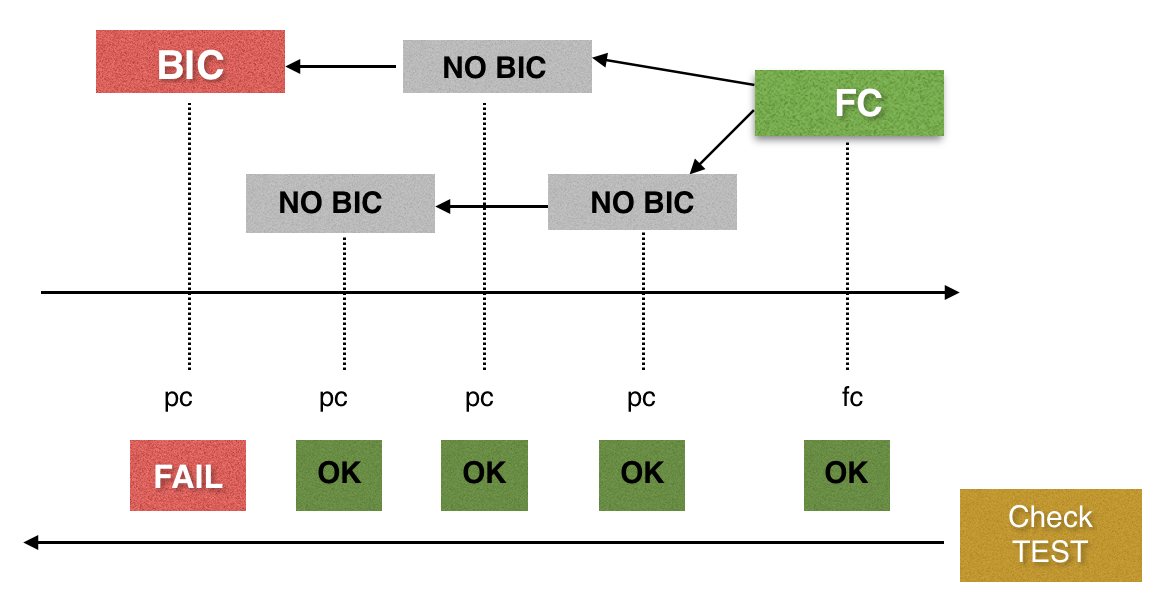
\includegraphics[height=4cm]{testrecursive.png}
\caption{Example of how we could find a candidate commit to be the  bug inducing change. Each version passes or not a test written after fixing the bug in the FC (fixing commit).}
\label{fig:test}      
\end{figure}

Next, we describe the methodology that we have used in our empirical experiments to find the origin of the malfunction in the software using a method based on lines and also based on tokens. 

Figure~\ref{fig:diagram} provides an overview of each step involved in our study and their outcomes.

\begin{figure}[ht]
\centering
%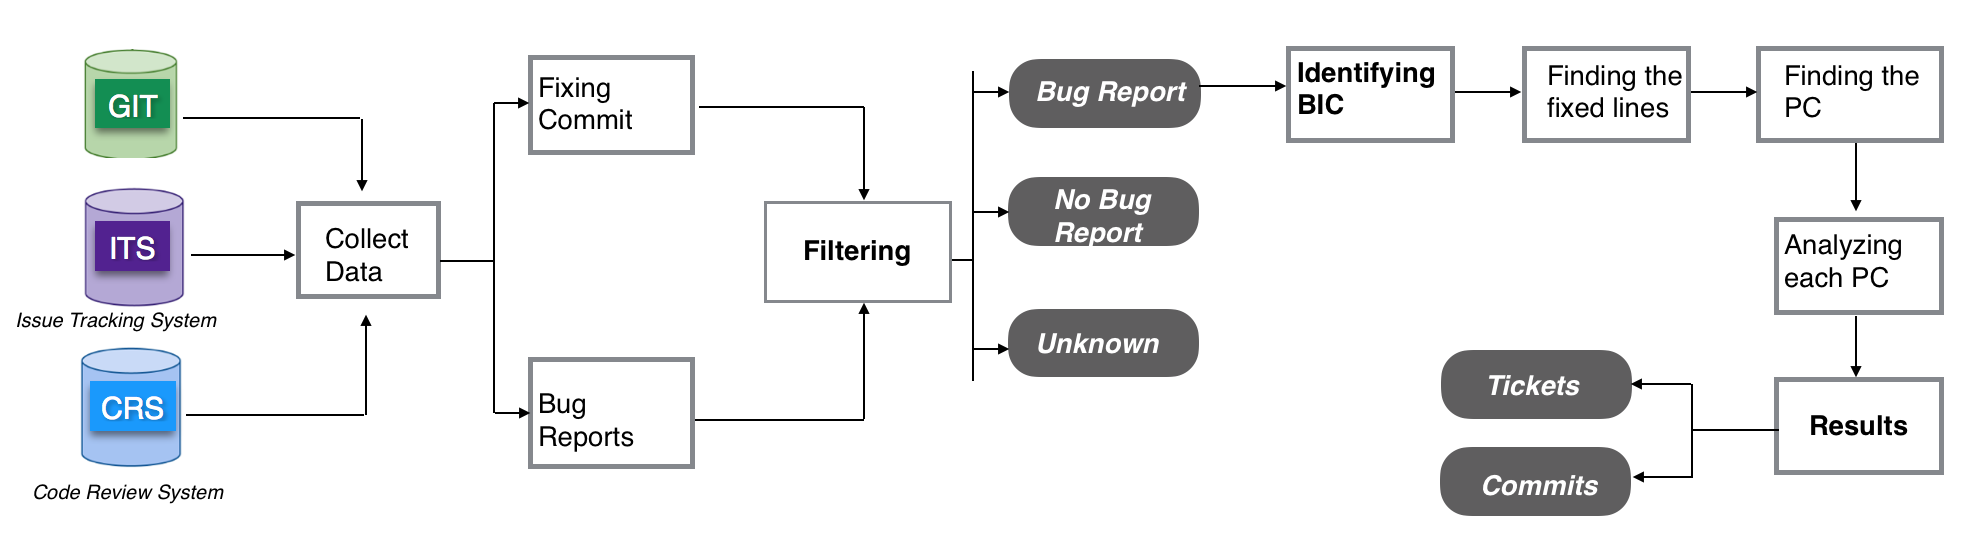
\includegraphics[width=\columnwidth]{diagram.png}
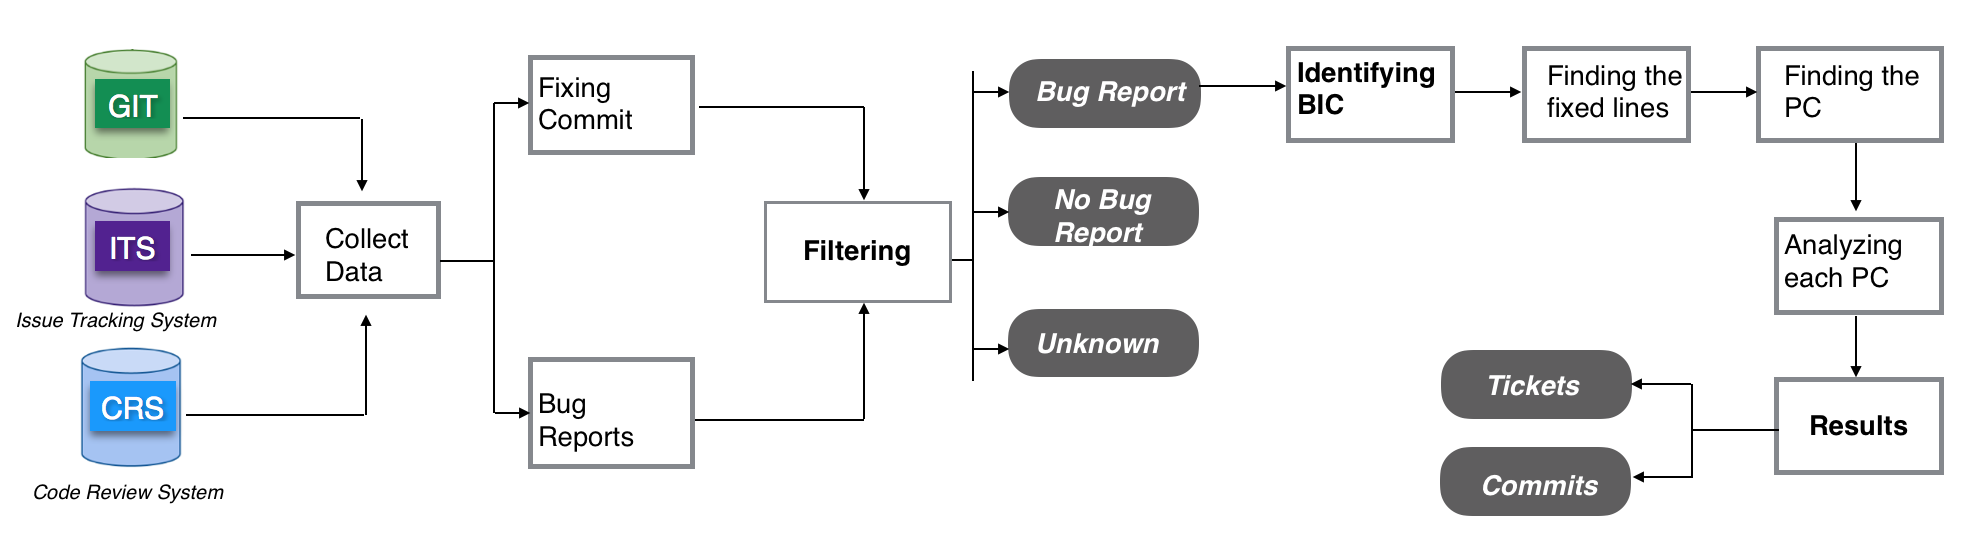
\includegraphics[height=3cm]{diagram.png}
\caption{Overview of the steps involved in our analysis. \emph{PC} refers to the immediately previous commit of a fixed line }
\label{fig:diagram}       % Give a unique label
\end{figure}

At the end of this step we have two main groups for each bug analyzed:
\begin{itemize}
	\item Group 1 : The bug has been always there, then the test will always fail.
	\item Group 2: The bug can be found using the test. Thus, we have two main reasons: (a) The test fails as we expected because the failure was due to a change in other part of the code that affects the code fixed or  the fixed line(s)/token(s) cannot be checked before because they didn't exists. (b) The test fails because a previous change (the immediately previous commit or an older commit) injected the bug.
\end{itemize}
\subsection{Results}

We have analyzed randomly 59 bug reports from each project, looking for the origin of a bug. Thus, after finding the line(s)/token(s) which fixed the bug in the 59 bug reports we found that almost all bug reports analyzed were in group 2, so we could be able to locate the buggy version for each bug report. Table~\ref{fig:tableI} shows the percentage of bug reports belong to groups 1, 2(a) or 2(b) using the line and token method.

\begin{table}[!t]
\renewcommand{\arraystretch}{1.3}
\caption{classification of each ticket analyzed depending on the nature of its bug}
\label{fig:tableI}
\centering
\begin{tabular}{|c||c||c|c|c|}
\hline
 & Nova(L) & ES(L)& Nova(T) & ES(T) \\
\hline
Group 1 & 7 (12\%) & 8 (13\%)& 7 (12\%) & 7 (12\%)\\
\hline
Group 2(a) & 29 (49\%) & 29 (49\%)& 33 (56\%) & 33 (56\%)\\
\hline
Group 2(b) & 23 (39\%) & 22 (37\%)& 19 (32\%) & 19 (32\%)\\
\hline
\end{tabular}
\end{table}

Additionally, in those cases where the test fails as we expected and the ticket does not present a bug inducing change into the previous commits, we are able to present a short classification of the main reasons: (1) Changes to APIs, such as the addition of an argument, (2) Changes in external artifact, (3) New lines added in the fixing commit.

Furthermore, our research shows evidence that assuming that the previous commit is where the cause of a bug can be found does not hold for a significant fraction of bugs. The most common reasons for the previous commit was not a bug inducing change in the projects are: (1) Variable renaming, (2) Changes done by the bug fixing commit in a clean line, (3) Refactoring of the code in some lines.

\subsection{New Metrics}

Furthermore, once we know exactly the moment when the bug was inserted we are able to calculate metrics such as the Time To Fix (TTF), the Time To Review (TTR), the Time To Notify (TTN) a bug or the fix-effort to improve code quality and to study the relationship between them. Currently, we could compute the TTF, TTR and the fix effort by locating with the SZZ the bug introduction change. However our proposal improve these metrics since they are computed from the precise moment when the bug was injected and not from the main assumption that the SZZ makes. We believe that the study of such metrics may prevent the injection of bugs in the future and help us understanding and measuring the software evolution.

Figure~\ref{fig:metrics} provides a visual explanation of the metrics that we propose.

\begin{figure}[ht]
\centering
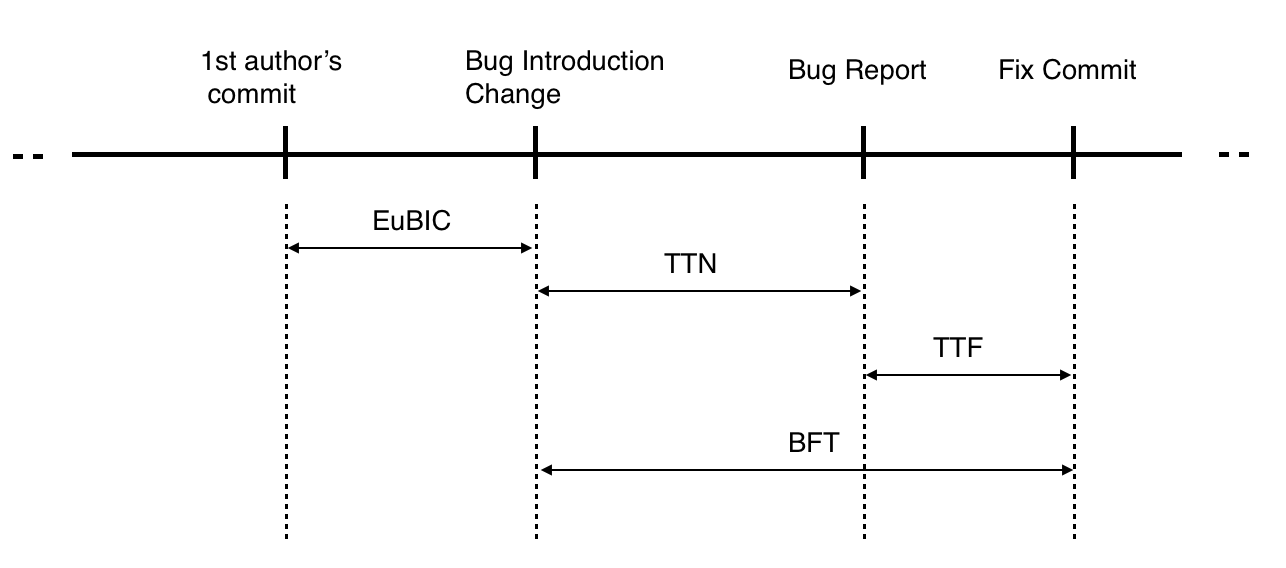
\includegraphics[height=4cm]{metrics.png}
\caption{Visualization of the periods under study: EuBIC, TTN, TTF, BFT.}
\label{fig:metrics}       % Give a unique label
\end{figure}

\begin{itemize}
\item{Experience until Bug Introducing Change (EuBIC):}
Experience measures in days of the author inserting the bug at the moment of doing the commit. 
\item{Time To Notify (TTN):}
Time in days since the bug inducing commit was merged into the master branch until some developer notified the bug and reported it in the bug tracking system. 
\item{Time To Fix (TTF):}
Period in days from the notification of a bug report to when it was closed with a fixing commit.
\item{Bug Fixing Time (BFT):}
Time in days from the date of the bug inducing change to the fixing commit date.
\end{itemize}


\section{Conclusions and further research}

In this paper we present two of our ongoing research works, the first describes a new approach to locate the origin of a bug based on the idea of testing each previous version until find the version that causes the malfunction of the code. This way, we could reduce the false positives and also find the missing false negatives that SZZ causes. This empirical study gives cause for understanding how metrics extracted from the precise location of a bug are related to the maintenance and evolution of a software.

Our second research provides deep insight on the credibility and use of the most known algorithm to locate the line(s) that injected the bug into the source code. With a systematic literature review of this algorithm we try to understand how other studies used it and how we authors mitigate their limitations.

A future line could be the full automation of the methodology used in this paper, that would provide software projects with a valuable tool for understanding how bugs are introduced, and therefore calculate these metrics for mitigation.

%\bibliographystyle{alpha} 
%\bibliography{samplebib}
%inline the .bbl file directly for mailing to authors.

\begin{thebibliography}{Com79}

\bibitem[sliwerski2005]{sliwerski2005changes}
{\'S}liwerski, Jacek and Zimmermann, Thomas and Zeller, Andreas
\newblock When do changes induce fixes?.
\newblock {\em Proceedings of the 2005 International Workshop on Mining software repositories}, 1--5, 2005.

\bibitem[prechelt2014]{prechelt2014software}
Prechelt, Lutz and Pepper, Alexander.
\newblock {\em Why software repositories are not used for defect-insertion circumstance analysis more often: A case study -- Volume 56, 1377--1389 / Information and Software Technology}.
\newblock Elsevier, 2014.

%\bibitem[german2009]{german2009change}
%German, Daniel M and Hassan, Ahmed E and Robles, Gregorio
%\newblock {\em Change impact graphs: Determining the impact of prior codechanges -- Volume 51, 1394--1408 / Information and Software Technology}.
%\newblock Elsevier, 2009.

\bibitem[hata2010]{hata2010fault}
Hata, Hideaki and Mizuno, Osamu and Kikuno, Tohru
\newblock {\em Fault-prone module detection using large-scale text features based on spam filtering -- Volume 15, 147--165 / Empirical Software Engineering}.
\newblock Springer, 2010.

\bibitem[mizuno2010]{mizuno2010prediction}
Mizuno, Osamu and Hata, Hideaki
\newblock {\em Prediction of fault-prone modules using a text filtering based metric -- Volume 4, 43--52 / International Journal of Software Engineering and Its Applications}.
\newblock 2010.

\bibitem[da2016]{da2016framework}
da Costa, Daniel Alencar and McIntosh, Shane and Shang, Weiyi and Kulesza, Uira and Coelho, Roberta and Hassan, Ahmed
\newblock {\em A Framework for Evaluating the Results of the {SZZ} Approach for Identifying Bug-Introducing Changes / IEEE Transactions on Software Engineering}.
\newblock IEEE, 2016.


\end{thebibliography}

\end{document}

